\section{Introduction}
\label{sec:intro}

The energy consumption due to buildings (both residential and commercial)
is estimated to be 20\% to 40\% of the total energy usage in
developed countries~\cite{pop08}, and
lighting and heating are two significant components of this energy
consumption~\cite{keh05}.
Natural light (i.e., sunlight) is a readily available resource that
can contribute to both the illumination~\cite{Leslie03}
and heating~\cite{Lunde80} of structures,
yet in the vast majority of circumstances, its use is limited to
passive modalities.  For example, daylighting (the use of natural
light for illumination) design is dominated by passive window positioning
and configuration~\cite{vgf+13} rather than active control mechanisms
(see~\cite{kt16} for the few counterexamples).
Heating systems that use sunlight do frequently use actively-controlled mirrors
for tracking the relative position of the sun.

We propose to investigate the ability to effectively utilize actively
controlled catoptric (mirror) surfaces to benefit the illumination and
heating of buildings.  Computer-based control of the dynamic positioning of
individual mirrors, and computer-based management of the sunlight
(as a resource), clearly put a system such as this within the scope
of traditional cyber-physical systems.

Figure~\ref{fig:amp} is an image of a prototype catoptric surface
(called AMP) that was designed, fabricated, and installed through an
undergraduate architecture studio taught by Co-PI C.~Ahrens. The installation
redirects light from gable ends of an existing building into the darker
recesses of the atrium to create better natural lighting where it is desired.
In this installation, the mirror positions are fixed.

\begin{figure}[ht]
\centering
\subfloat[\mbox{ }]{
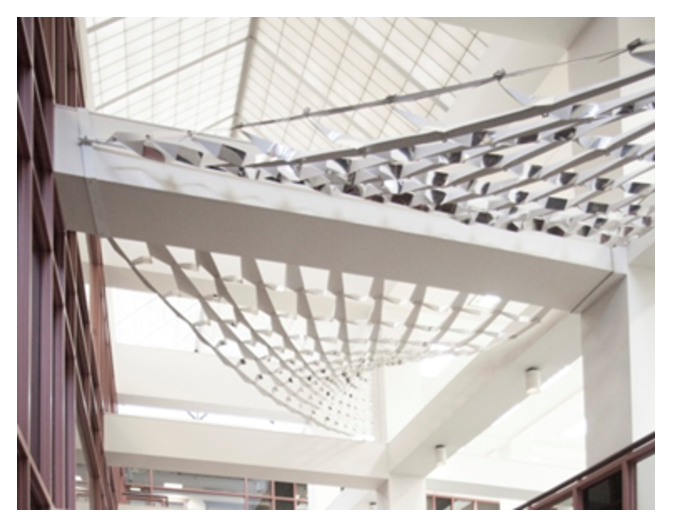
\includegraphics[width=0.5\linewidth]{figures/amp}
\label{fig:amp}}
\qquad \qquad
\subfloat[\mbox{ }]{
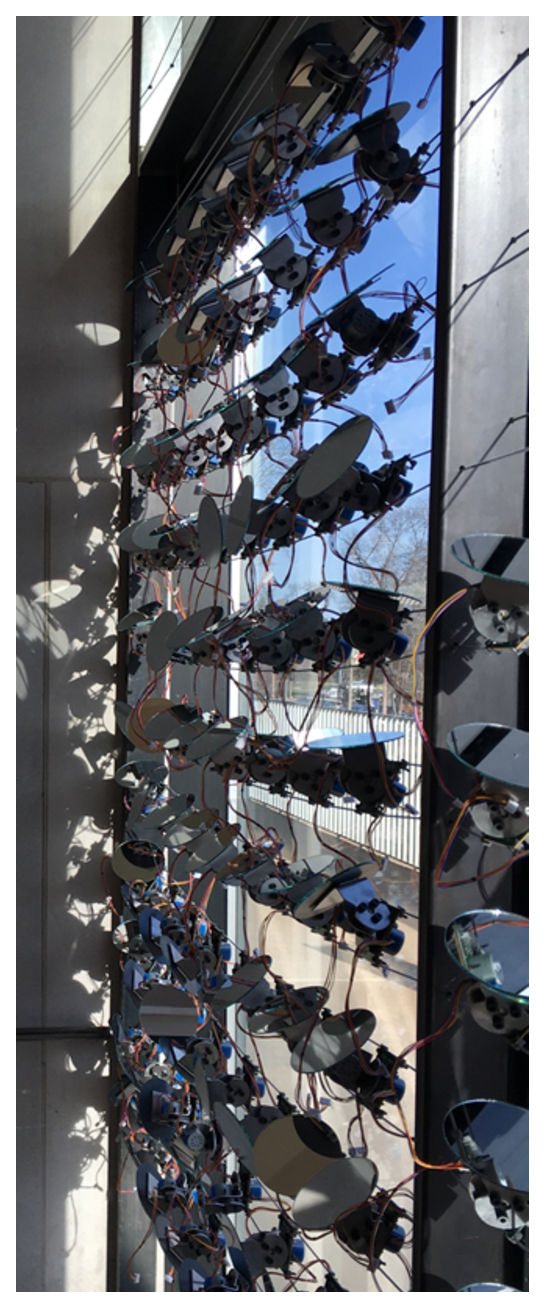
\includegraphics[width=0.16\linewidth]{figures/steinberg}
\label{fig:steinberg}}
\caption{Catoptric system prototypes.
(a)~\emph{AMP}, TRex building, St. Louis, MO.
(b)~\FIXME{name?}, Steinberg Hall, St. Louis, MO.
}
\label{fig:proto}
\end{figure}

In the next generation of this system, which is currently under construction,
over 600 mirrors are under active, 2-axis, microprocessor-based control and
therefore can be pointed in different directions dynamically as desired
over time. This installation is on the south wall of the Steinberg Hall
atrium (on
the campus of Washington University in St. Louis), and a subset of the
mirrors are shown in Figure~\ref{fig:steinberg}.

The ability to actively control the dynamic position of each mirror provides
for unprecidented capacity to position the available natural light where
it is desired.  This can easily change over time, as the usage of the
physical space changes.

The proposed research advances the investigation of reflected light by
designing specific intensities in some areas and dissipated lighting
conditions in other areas according to pre-determined, yet adjustable,
image-based maps. The maps can consist of any raster image and generate the
target positions for the reflected light in a space.  The image is sampled
according to intensity (black to white) to determine the density
of target points where the higher the value, the denser the resulting
field of points. Using an image-based map allows users to visualize
zones of intensity in an interior space prior to the mirrors reflecting
the daylight. Any user is capable of supplying or creating the image
to be used for the map, thus encouraging user control and interaction with
the system. The engagement of any member of a community on the creation
of that image has an impact on the entire community~\cite{BS13} and
encourages dialog about the quality and quantity of light within their
environment. 

Given the desire to control natural light (sunlight) via a catoptric surface,
repurposing it for illumination and/or thermal management, a number of
cruicial cyber-physical system issues must be addressed.
This research will investigate the following questions:
\begin{enumerate}

\item \emph{What are the qualitative and quantitative benefits
that can be achieved for bulding daylighting and thermal management
through the use of catoptric systems?}

Issues within this question include the ability to articulate the benefits
and to quantify them effectively.  Clearly, we are in the domain
of multi-objective control, so the relationship between the competing
goals must also be articulated and quantified. We intend to investigate
the use of Markov Decision Processes (MDPs) as an approach to
the multi-objective control problem, recognizing that maximization
(of an objective function) in expectation is a robust way to acknowledge
the inherent uncertainty of future events (whether it be sunlight availability,
lighting demand, or any other effect that is stochastic in nature).

\item \emph{How do we provide for the safety, reliability, maintainability, and
continued efficacy of these systems?}

Even with an ideal multi-objective control system in place, the system as
a whole has limited usefulness if these additional requirements are not
dealt with in an effective way.  Initially, just consider the issue of
safety: highly concentrated sunlight aimed at a heat collector (important
when harvesting energy for thermal management purposes) can be quite harmful
if inadvertently aimed at humans. 

Each of these system-level requirements must ultimately be included within
the optimization problem formulation, either as constraints (e.g., for
safety) or as additional objectives (e.g., reliability and/or maintainability).
Fortunately, the MDP formalism is well suited to the addition of concerns
such as these (especially those with a stochastic nature, as reliability
and maintainability tend to be).

\item \emph{Can we design abstractions that encapsulate subsystems for
effective reuse?}

A pair of immediate possibilities come to mind. Separating the concerns
of low-level control (e.g., of mirror positions) and high-level system
management (how the available light resource should be allocated) is one
option.  The low-level control subsystem can be encapsulated into a reusable
component, applicable to any number of physical positioning applications.
Similarly, a high-level management system (e.g., based upon MDP theory)
could also be encapsulated in a resuable component, applicable to any
number of other stochastic optimization problems.
Ultimately, we would like to generalize the above into abstractions that can be
leveraged more broadly for arbitrary cyber-physical systems development.

\end{enumerate}

\FIXME{Brief description of who we are and what we've done.}
